% ===================== 担当C =====================
\section{担当C — 楽譜・演奏制御}

\subsection{機能一覧}
担当Cでは，以下の2点を担当する．
\begin{enumerate}
  \renewcommand{\labelenumi}{(\arabic{enumi})}
  
\item \textbf{楽譜データの作成}

\item \textbf{Arduino-Processing間の通信システムの設計・実装}

\end{enumerate}

各楽器の演奏開始タイミングは，親機Processingから送信される輝度キューによって決定される．発表当日にProcessingの楽器指定ボタンから順番に入力することで各子機へスタートキューが送られる．演奏予定順序を表\ref{offset01}に示す．なお，最終的な順序は試聴によって調整を行う．
\begin{table}[H]
  \centering
  \caption{演奏予定順序（親機から動的に指示）}
  \label{offset01}
  \begin{tabular}{|c|c|c|}
\hline
楽器 & 演奏開始 & パート \\\hline \hline
ハイハット・シンバル & 0小節目 & リズム１ \\ \hline
バス・スネア & 0小節目 & リズム２ \\ \hline
鉄琴 & 2小節目 & 主旋律１ \\ \hline
ピアノ & 4小節目 & 主旋律２ \\ \hline
トランペット & 6小節目 & 主旋律３ \\ \hline
  \end{tabular}  
\end{table}
\FloatBarrier

演奏テンポは表\ref{テンポ}の通りである．\\
\begin{table}[h]
  \centering
  \caption{演奏テンポ一覧表}
  \label{テンポ}
  \begin{tabular}{|c|c|}
\hline
区間 & テンポ  \\\hline \hline
開始〜14小節（一周目演奏終了） & 80bpm \\ \hline
15小節目（二周目演奏開始）以降 & 104bpm  \\ \hline


  \end{tabular}  
\end{table}
\FloatBarrier

演奏用Arduino-Processing 間の通信は有線接続によってシリアル通信を行う．ArduinoからProcessingへ送信する内容一覧は表\ref{serial}に記す．

\begin{table}[h]
  \centering
  \caption{シリアル通信パケット仕様}
  \label{serial}
  \begin{tabular}{|c|c|c|c|c|}
\hline
バイト & フィールド名& 内容& 型 & 範囲  \\\hline \hline
0&NOTE\_OFF&前の音の終了&uint8&true = 1，false = 0 \\ \hline
1 & NOTE & 音名インデックス & uint8 &   0〜127（255 = 休符）\\ \hline
2 & VEL & 音の強さ & uint8 &   0〜127\\ \hline
  \end{tabular}  
\end{table}
\FloatBarrier

\subsection{システム構成図}
担当Cのシステム構成図は図\ref{system}の通りである．


\begin{figure}[H]
    \centering
    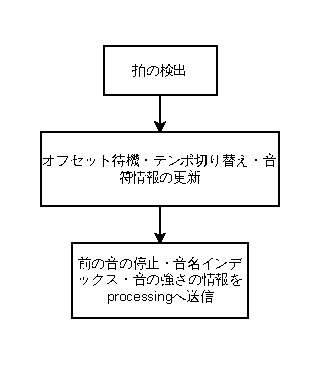
\includegraphics[,width=0.8\linewidth, keepaspectratio]{figures/tantoC/system.drawio.pdf}
    \caption{担当Cシステム構成図}
    \label{system}
\end{figure}



%\subsection{状態遷移図}

%\figspace[4]{状態遷移図を挿入}
